\documentclass[addpoints, 12pt]{exam}%, answers]
\usepackage[utf8]{inputenc}
\usepackage[T1]{fontenc}

\usepackage{lmodern}
\usepackage{arydshln}
\usepackage[margin=2cm]{geometry}

\usepackage{enumitem}
\usepackage{multicol}

\usepackage{enumerate}
\usepackage{breqn}
\usepackage{parskip}

\usepackage{amsmath, amsthm, amsfonts, amssymb}
\usepackage{graphicx}
\usepackage{tikz}
\usetikzlibrary{arrows,calc,patterns}
\usepackage{pgfplots}
\pgfplotsset{compat=newest}
\usepackage{url}
\usepackage{multicol}
\usepackage{thmtools}

\usepackage{caption}
\usepackage{subcaption}

\usepackage{pifont}

% MATH commands
\newcommand{\bC}{\mathbb{C}}
\newcommand{\bR}{\mathbb{R}}
\newcommand{\bN}{\mathbb{N}}
\newcommand{\bZ}{\mathbb{Z}}
\newcommand{\bT}{\mathbb{T}}
\newcommand{\bD}{\mathbb{D}}

\DeclareMathOperator{\dom}{dom}

\newcommand{\spc}{\vspace*{0.5cm}}
\CorrectChoiceEmphasis{\color{red}}

\begin{document}
\noindent \hrulefill \\
	MATH-241 Calculus I \hfill Created by Rukiyah Walker\\
	Homework 15 \hfill Spring 2023\\ \vspace*{-1cm}
 
	\noindent\hrulefill

\qformat{\rule{0.3\textwidth}{.4pt} \begin{large}{\textsc{Question}} \thequestion \end{large} \hspace*{0.2cm} \hrulefill \hspace*{0.1cm} \textbf{(\totalpoints\hspace*{0.1cm} pts)}}

\begin{questions}

\vspace*{0.5cm}

\question[1]

Suppose you want to find the area between the two curves in this graph. You need both $\Delta x$ and the height between each curve. What is the formula to find the height between each curve?
\begin{minipage}{0.5\textwidth}
\begin{choices}
\choice  $f(x) = g(x)$\vspace*{10pt}
\choice $f'(x) - g'(x)$ \vspace*{10pt}
\CorrectChoice $f(x) - g(x)$ \vspace*{10pt}
\choice $f(x) + g(x)$ \vspace*{10pt}
\end{choices}
\end{minipage}
\hspace*{1cm}
\begin{minipage}{0.35\textwidth}
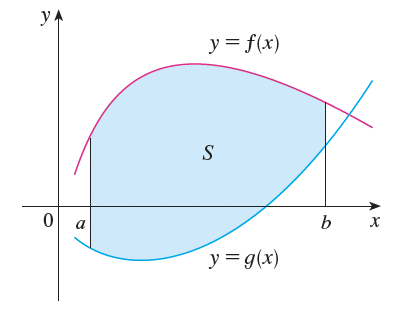
\includegraphics[width=1\textwidth]{HW15graph.png}
\end{minipage}

\spc

\question[1]

Write the area between the two curves bounded by the lines $x = a$ and $x = b$ in question 1 as an integral. 

\begin{multicols}{2}
\begin{choices}
\CorrectChoice $\int_{a}^{b} [f(x) - g(x)]dx$
\choice $\int_{a}^{b} [f(x) - g(x)\Delta x]dx$
\choice $\int_{a}^{b} [f'(x) - g'(x)]dx$
\choice $\int_{a}^{b} [f(x) + g(x)\Delta x]dx$
\end{choices}
\end{multicols}

\spc

\question[1]

Suppose you want to find the area of the region enclosed by the two parabolas $y = x^2$ and $y = 2x - x^2$. Find the points of intersection of the two parabolas (the zeros). This will be the lower, $a$, and upper bounds, $b$, of the integrand.

\begin{multicols}{2}
\begin{choices}
\choice $a = 1$, $b = 2$
\CorrectChoice $a = 0$, $b = 1$
\choice $a = 2$, $b = 4$
\choice $a = 0$, $b = 2$
\end{choices}
\end{multicols}

\spc

\question[1]

Write the total area between the two curves in question 3 in integral form.

\begin{multicols}{2}
\begin{choices}
\choice $\int_{0}^{2} 2x^2 - 2x dx$
\choice $\int_{2}^{4} 2x dx$
\choice $\int_{1}^{2} x^2 dx$
\CorrectChoice $\int_{0}^{1} 2x - 2x^2 dx$
\end{choices}
\end{multicols}

\newpage

\question[1]

Suppose you want to find the volume of the solid obtained by rotating the region bounded by $y = x + 1$, $y = 0$, $x = 2$, and $x = 0$ about the $x$-axis. By rotating around the $x$-axis, you get a new solid shape which can be split into multiple disks. What is the radius of the disk? 

\begin{minipage}{0.5\textwidth}
\begin{choices}
\choice $r = 2$ \vspace*{10pt}
\choice $r = x - 1$\vspace*{10pt}
\CorrectChoice $r = x + 1$ \vspace*{10pt}
\choice $r = 0$ \vspace*{10pt}
\end{choices}
\end{minipage}
\hspace*{1cm}
\begin{minipage}{0.35\textwidth}
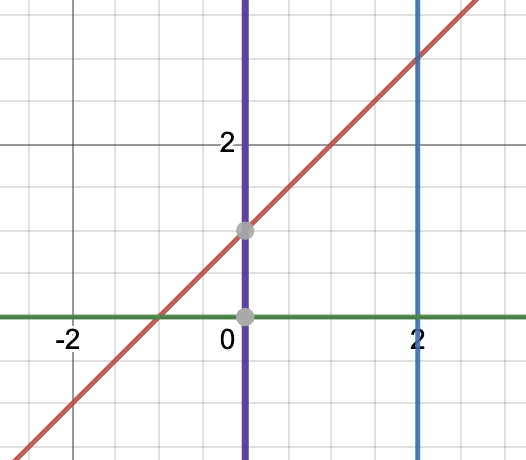
\includegraphics[width=1\textwidth]{HW15graph2.png}
\end{minipage}

\spc

\question[1]

Write the volume of the solid in question 5 in integral form.

\begin{multicols}{2}
\begin{choices}
\choice $\int_{-1}^{2} \pi(2x)^2dx$
\CorrectChoice $\int_{0}^{2} \pi(x+1)^2dx$
\choice $\int_{0}^{2} \pi(x-1)^2dx$
\choice $\int_{-1}^{2} \pi(x-1)^2dx$
\end{choices}
\end{multicols}

\spc

\question[1]

Suppose you want to find the volume of the solid obtained by rotating the region bounded by $x = 2\sqrt{y}$, $x = 0$, and $y = 9$ about the $y$-axis. What is the radius of the disk of the resulting solid?

\begin{minipage}{0.5\textwidth}
\begin{choices}
\choice $r = y^2$ \vspace*{10pt}
\choice $r = 2x^2$ \vspace*{10pt}
\choice $r = 2y$ \vspace*{10pt}
\CorrectChoice $r = 2\sqrt{y}$ \vspace*{10pt}
\end{choices}
\end{minipage}
\hspace*{1cm}
\begin{minipage}{0.35\textwidth}
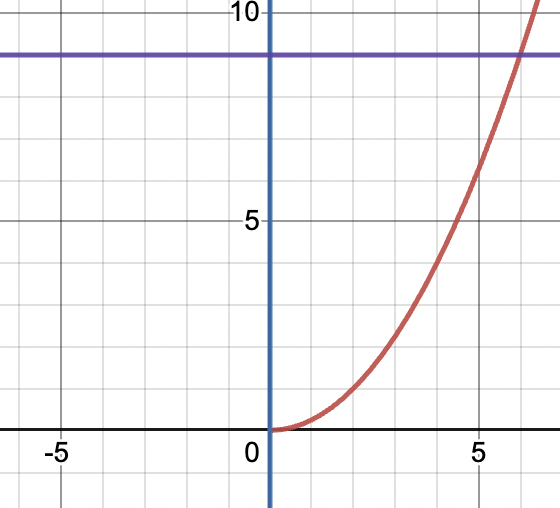
\includegraphics[width=1\textwidth]{HW15graph3.png}
\end{minipage}

\spc

\question[1]

Write the volume of the solid in question 7 in integral form.

\begin{multicols}{2}
\begin{choices}
\CorrectChoice $\int_{0}^{9} \pi (2\sqrt{y})^2dy$
\choice $\int_{0}^{6} \pi (\frac{x}{2})^2dx$
\choice $\int_{0}^{9} \pi (\frac{x}{2})^2dy$
\choice $\int_{0}^{6} \pi (2\sqrt{y})^2dx$
\end{choices}
\end{multicols}


\question[1]

Suppose you use the method of cylindrical shells to find the volume generated by rotating the region bounded by $y = x^2$ and $y = 6x - 2x^2$ about the $y$-axis. What is the height of a shell?

\begin{minipage}{0.5\textwidth}
\begin{choices}
\choice $6x - 2x^2$ \vspace*{10pt}
\CorrectChoice $6x-3x^2$ \vspace*{10pt}
\choice $\sqrt{y}$ \vspace*{10pt}
\choice $x^2$ \vspace*{10pt}
\end{choices}
\end{minipage}
\hspace*{1cm}
\begin{minipage}{0.35\textwidth}
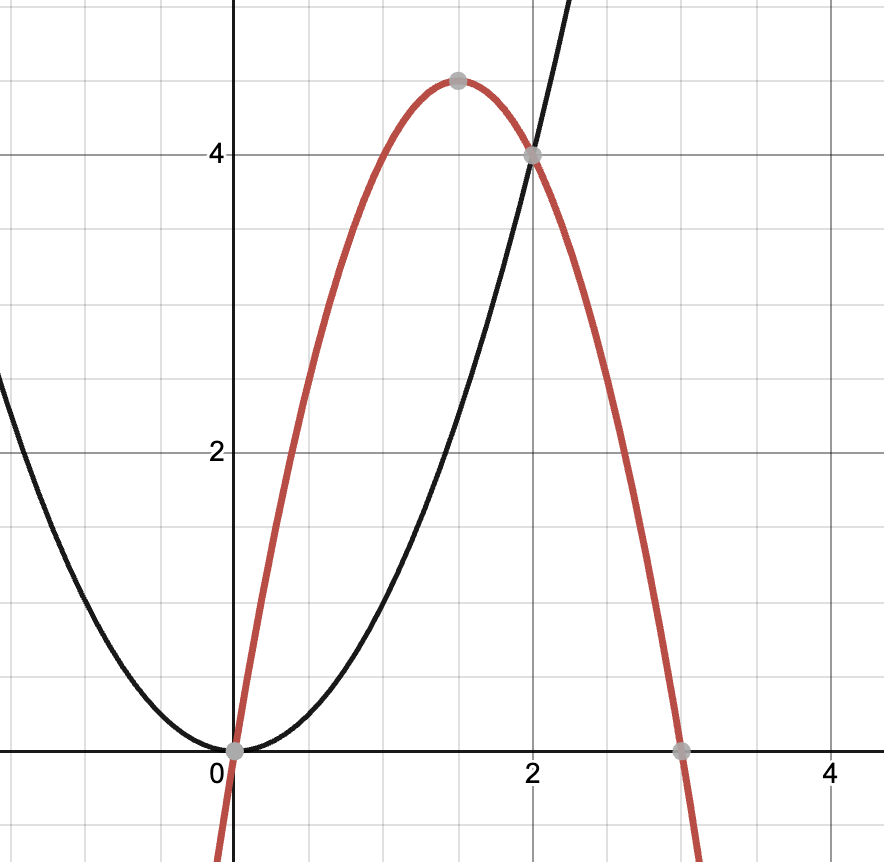
\includegraphics[width=1\textwidth]{HW15graph4.png}
\end{minipage}


\spc

\question[1]

 Write the volume of question 9 in integral form.

\begin{multicols}{2}
\begin{choices}
\choice $\int_{0}^{2} 2\pi x(6x-2x^2)dx$
\choice $\int_{0}^{5} 2\pi x\sqrt{y}dy$
\choice $\int_{0}^{5} 2\pi x^3dy$
\CorrectChoice  $\int_{0}^{2} 2\pi x(6x-3x^2)dx$
\end{choices}
\end{multicols}


\end{questions}
\end{document}
